\begin{frame}
    \begin{PointSix}{Learning Goals}
      \alert{Learning goals today:}
      \begin{itemize}
        \item Peak into applications
        \item Principals about magnetic fields (i.e., dipole field, $\vec{H}$,$\vec{B}$,$\vec{M}$,$\chi$)
        \item The Earth's magnetic field (T,H,D,I,..)
        \item The idea behind magnetic surveys.
      \end{itemize}
    \end{PointSix}
\end{frame}



\begin{frame}
  \begin{PointSix}{Example Applications}
    
    \includegraphics[width=\linewidth]{Figures/Magnetics/Pipeline_Guoetal2014_JApplPhysics.png}
  
    \tiny [Guo et al., 2014, J. Appl. Geophys.]
  \end{PointSix}
\end{frame}

\begin{frame}
  \begin{PointSix}{Example Applications}
    
    \includegraphics[width=\linewidth]{Figures/Magnetics/Archeology_CiminaleEtAl_2009_ArcheoSciences.jpg}
    %Dipole field removed. Information mirrors mostly crustal rock composition.
    \tiny [Ciminale et al., 2009, Archeosciences.]
  \end{PointSix}
\end{frame}

\begin{frame}
  \begin{PointSix}{Example Applications}
    
    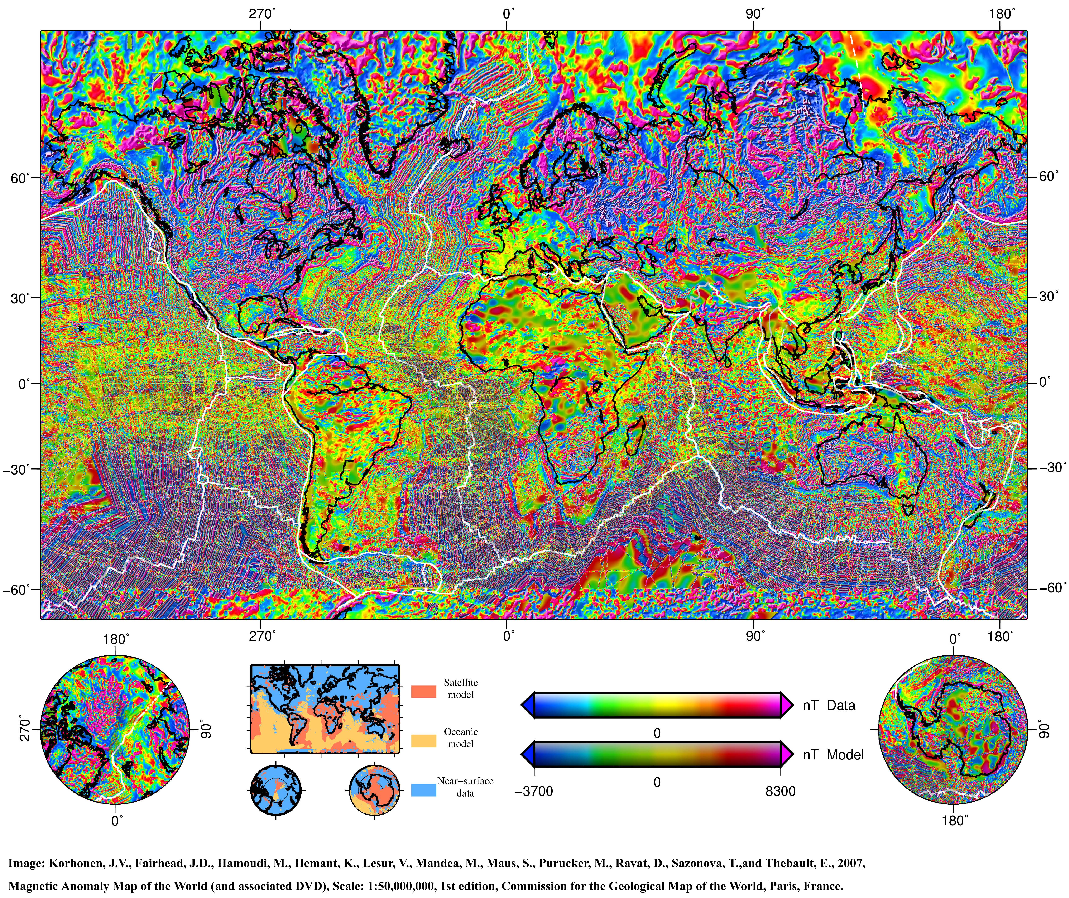
\includegraphics[width=\linewidth]{Figures/Magnetics/GlobalAnomalyMap_KorhonenEtAl_2007_CommissionGeologicalMapOfTheWorld.pdf}
    %Dipole field removed. Information mirrors mostly crustal rock composition.
    \tiny [Korhonen et al., 2007, C. Geolog. Map., Paris, France.]
  \end{PointSix}
\end{frame}

\begin{frame}
  \begin{PointSix}{Fundamentals}
    What causes a magnetic field? 
  \end{PointSix}
\end{frame}

\begin{frame}
  \begin{PointSix}{Fundamentals}
    What causes a magnetic field?
    \begin{itemize}
      \item Let's use an analog to the point mass in the gravity method
      \item Let's represent 'north' and 'south' poles with point charges
      \item Let's derive the potential $A$ of a pair of positive-negative point masses
      \item Let's get the field using $\vec{B} = \nabla A$
    \end{itemize} 
  \end{PointSix}
\end{frame}

\begin{frame}
  \begin{PointSix}{The magnetic dipole potential}
    %http://hyperphysics.phy-astr.gsu.edu/hbase/electric/dipole.html
    \begin{tikzpicture}
    
      \coordinate (Qm) at ( 0,0);
      \coordinate (Qp) at (5,0);
      \coordinate (Center) at (2.5,0);
      \coordinate (P) at (4,4);
      \draw[o-o,thick] (Qm) -- (Qp) node[midway, below] {$2l$};
      \draw[-o,thick] (Center) -- (P) node[midway, left] {$r$};
      \draw[-,thick] (Qm) -- (P) node[midway, left] {$r_1$};
      \draw[-,thick] (Qp) -- (P) node[midway, right] {$r_2$};
      \node at (Qm) [below = 1mm of Qm] {$'+'$};
      \node at (Qm) [below = 10mm of Qm] {\Large $\frac{p}{r
      _1}$};
      \node at (Qp) [below = 10mm of Qp] {\Large $-\frac{p}{r
      _2}$};
      \node at (Qp) [below = 1mm of Qp] {$'-'$};
      \node at (P) [right = 1mm of P] {$P$};
      \pic [draw, ->, "$\theta$", angle eccentricity=1.5] {angle = Qp--Center--P};
    \end{tikzpicture}

  \small Use 'magnetic' potential in analogy to gravity potential
  \end{PointSix}
\end{frame}

\begin{frame}
  %http://hyperphysics.phy-astr.gsu.edu/hbase/electric/dipole.html
  \begin{PointSix}{The magnetic dipole potential}
    \begin{align*}
      A & =  \frac{p}{r_1} - \frac{p}{r_2} \\
        & =  \frac{p(r_2-r_1)}{r_1r_2}
    \end{align*}
  \end{PointSix}
\end{frame}



\begin{frame}
  %http://hyperphysics.phy-astr.gsu.edu/hbase/electric/dipole.html
  \begin{PointSix}{The magnetic dipole potential: farfield}
    \begin{tikzpicture}
    
      \coordinate (Qm) at ( 0,0);
      \coordinate (Qp) at (3,0);
      \coordinate (Center) at (1.5,0);
      \coordinate (P) at (8,4);
      \draw[o-o,thick] (Qm) -- (Qp) node[midway, below] {$2l$};
      \draw[-o,thick] (Center) -- (P) node[midway, left] {$r$};
      \draw[-,thick] (Qm) -- (P) node[midway, left] {$r_1$};
      \draw[-,thick] (Qp) -- (P) node[midway, right] {$r_2$};
      \node at (Qm) [below = 1mm of Qm] {$'+'$};
      \node at (Qp) [below = 1mm of Qp] {$'-'$};
      \node at (P) [right = 1mm of P] {$P$};
      \pic [draw, ->, "$\theta$", angle eccentricity=1.5] {angle = Qp--Center--P};
    \end{tikzpicture}
    \begin{align*}
      A & =  \frac{p(r_2-r_1)}{r_1r_2} \qquad \text{for} \qquad r \gg l
    \end{align*}
     \end{PointSix}
\end{frame}

\begin{frame}
  %http://hyperphysics.phy-astr.gsu.edu/hbase/electric/dipole.html
  \begin{PointSix}{The magnetic dipole potential: farfield}
    \begin{tikzpicture}
    
      \coordinate (Qm) at ( 0,0);
      \coordinate (Qp) at (3,0);
      \coordinate (Center) at (1.5,0);
      \coordinate (P) at (8,4);
      \draw[o-o,thick] (Qm) -- (Qp) node[midway, below] {$2l$};
      \draw[-o,thick] (Center) -- (P) node[midway, left] {$r$};
      \draw[-,thick] (Qm) -- (P) node[midway, left] {$r_1$};
      \draw[-,thick] (Qp) -- (P) node[midway, right] {$r_2$};
      \draw[Karminrot,-,line width=0.75mm] (Qp) -- (2.28,1.14) ;
      \draw[Karminrot,|-|,line width=0.75mm] ([yshift=0.25cm,xshift=0.25]Qm) -- ([yshift=0.25cm,xshift=0.25] 2.28,1.14) node[midway,above,sloped] {$r_1-r_2$};
      \node at (Qm) [below = 1mm of Qm] {$'+'$};
      \node at (Qp) [below = 1mm of Qp] {$'-'$};
      \node at (P) [right = 1mm of P] {$P$};
      \pic [draw, ->, "$\theta$", angle eccentricity=1.5] {angle = Qp--Center--P};
    \end{tikzpicture}
    \begin{align*}
      A & =  \frac{p(r_2-r_1)}{r_1r_2} \approx \frac{2lp\cos(\theta)}{r^2} \qquad \text{for} \qquad r \gg l
    \end{align*}
  \end{PointSix}
\end{frame}

\begin{frame}
  %http://hyperphysics.phy-astr.gsu.edu/hbase/electric/dipole.html
  \begin{PointSix}{The magnetic dipole potential: farfield}
    \begin{tikzpicture}
    
      \coordinate (Qm) at ( 0,0);
      \coordinate (Qp) at (3,0);
      \node at (Qp) [right = 1mm of Qp] {$\vec{m}=2\vec{l}p$ (dipole moment)};
     
      \draw[o->o,thick] (Qm) -- (Qp) node[midway, below] {$2\vec{l}$};
      \draw[o->o,thick] ([yshift=1cm] Qm) -- ([yshift=2cm] Qp) node[midway, below] {$2\vec{l}$};
        \end{tikzpicture}
    \begin{align*}
      A & =  \frac{p(r_2-r_1)}{r_1r_2} \\
      &\approx \frac{2lp\cos(\theta)}{r^2} \\
      &= \frac{|\vec{m}|\cos(\theta)}{r^2}
    \end{align*}
  \end{PointSix}
\end{frame}
\begin{frame}
  %http://hyperphysics.phy-astr.gsu.edu/hbase/electric/dipole.html
  \begin{PointSix}{The magnetic dipole field}
    In analogy to the gravity potential:
    \begin{align*}
      \vec{B} & = -\nabla A \\
         &\approx -\nabla \frac{|\vec{m}|\cos(\theta)}{r^2} \\
         & = \frac{|m|}{r^3}\left(2\cos(\theta)\hat{r}+\sin(\theta)\hat{theta}\right)
    \end{align*}
    \small (Derivation in Exercises.)
  \end{PointSix}
\end{frame}


\begin{frame}
  \begin{PointSix}{Mathematical technicalities}
    \includegraphics[width=0.75\linewidth]{Figures/Magnetics/SphericalCoordinates_Reversed.pdf}
  \end{PointSix}
\end{frame}

\begin{frame}
  %http://hyperphysics.phy-astr.gsu.edu/hbase/electric/dipole.html
  \begin{PointSix}{Mathematical technicalities}
    \small Unlike cartesian coordinates, the unit vectors in polar coordinates ($\hat{\theta},\hat{\phi}$ not $\hat{r}$) are functions of positions. Therefore the derivatives take a different form in different coordinate systems.
    $$
    \nabla A = \hat{r}\frac{\partial}{\partial r} + \hat{\theta} \frac{1}{r}\frac{\partial}{\partial \theta}
    $$
    $$
    \nabla \cdot \vec{B} = \frac{1}{r^2}\frac{\partial}{\partial r}\left(r^2B_r \right)+\frac{1}{r\sin(\theta)}\frac{\partial}{\partial \theta}\left(\sin(\theta) B_\theta \right)
    $$
    \small No need to be scared. Totally doable with some exercises.
  \end{PointSix}
\end{frame}

\begin{frame}
  %http://hyperphysics.phy-astr.gsu.edu/hbase/electric/dipole.html
  \begin{PointSix}{The dipole field visualized}
    \begin{tikzpicture}
      \node[anchor=south west,inner sep=0] at (0,0) {\includegraphics[width=\linewidth]{Figures/Magnetics/DipoleExported.png}};
      %\draw[red,ultra thick,rounded corners] (5,3) rectangle (9.4,6.2);
      \draw[->,line width=0.75mm,pink] (4.5,3.5) -- (5.0,6) node[midway, right] {$\vec{m}$};
    \end{tikzpicture}
  \end{PointSix}
\end{frame}
\begin{frame}
  %http://hyperphysics.phy-astr.gsu.edu/hbase/electric/dipole.html
  \begin{PointSix}{The dipole field visualized}
    \begin{tikzpicture}
      \node[anchor=south west,inner sep=0] at (0,0) {\includegraphics[width=\linewidth]{Figures/Magnetics/DipoleRot.png}};
      %\draw[red,ultra thick,rounded corners] (5,3) rectangle (9.4,6.2);
      \draw[->,line width=0.75mm,pink,rotate around={-35:(4.75,4.75)}] (4.5,3.5) -- (5.0,6) node[midway, right] {$\vec{m}$};
    \end{tikzpicture}
  \end{PointSix}
\end{frame}
\begin{frame}
  %http://hyperphysics.phy-astr.gsu.edu/hbase/electric/dipole.html
\begin{PointSix}{The dipole field visualized}
    \begin{tikzpicture}
      \node[anchor=south west,inner sep=0] at (0,0) {\includegraphics[width=\linewidth]{Figures/Magnetics/DipoleRot2.png}};
      %\draw[red,ultra thick,rounded corners] (5,3) rectangle (9.4,6.2);
      \draw[->,line width=0.75mm,pink,rotate around={-142:(4.75,4.75)}] (4.5,3.5) -- (5.0,6) node[midway, right] {$\vec{m}$};
    \end{tikzpicture}
  \end{PointSix}
\end{frame}

\begin{frame}
\begin{PointSix}{Dipole summary}
  \begin{itemize}
    \item The dipole approach is simplest option because there are \alert{no magnetic monopoles}. 
    \item The dipole field has closed field lines and is oriented with the dipole moment $\vec{m}$.
    \item The dipole field is the basic 'unit' in magnetics.
  \end{itemize}
\end{PointSix}
\end{frame}

\begin{frame}
  \begin{PointSix}{Fundamentals}
    What causes a magnetic field? 
    \\
    \alert{Electric currents!}
    \includegraphics[width=0.8\linewidth]{Figures/Magnetics/DipoleCurrentLoop1.pdf}
  \end{PointSix}
\end{frame}

\begin{frame}
  \begin{PointSix}{Fundamentals}
    What causes a magnetic field? 
    \\
    \alert{Electric currents!}
    \includegraphics[width=0.8\linewidth]{Figures/Magnetics/DipoleCurrentLoopSide.pdf}
  \end{PointSix}
\end{frame}

\begin{frame}
  \begin{PointSix}{Dipole summary}
    \begin{itemize}
      \item A closed loop with a current is the source of a dipole field (and the calculation with positive/magnetic monopoles is a trick that makes it easier. Alternatively use Bio-Savart or a multipole expansion.)
    \end{itemize}
  \end{PointSix}
  \end{frame}

  \begin{frame}
    \begin{PointSix}{Magnetic field of the Earth}
      \includegraphics[width=0.99\linewidth]{Figures/Magnetics/MagneticFieldEarth_PReid_Edinburgh.png}

      \tiny [P. Reid, Univ. Edinburgh, UK]
    \end{PointSix}
  \end{frame}


  \begin{frame}
    \begin{PointSix}{Magnetic field of the Earth}
      \begin{itemize}
        \item Earth's magnetic field is to a good approximation a dipole field (in the absence of near-surface anomalies).
        \item The origin of this field is deep in Earth's interior (conduction currents in outer mantel).
        \item The dipole moment is not parallel to rotation axis but shift. Hence there is an offset between magnetic and geographic poles.
      \end{itemize}
    \end{PointSix}
    \end{frame}

    \begin{frame}
    \begin{PointSix}{Magnetic field of the Earth}
      \begin{itemize}
        \item North seeking end of magnetic needles dips downwards in northern hemisphere.
        \item South seeking end of magnetic needles dips downwards in southern hemisphere.
      \end{itemize}
    \end{PointSix}
    \end{frame}

    \begin{frame}
      \begin{PointSix}{Magnetic field of the Earth}
        \includegraphics[width=0.99\linewidth]{Figures/Magnetics/Coordinates.png}
      \end{PointSix}
    \end{frame}

    \begin{frame}
      \begin{PointSix}{Magnetic field of the Earth}
        \small
          T: total field ($T^2=H^2+Z^2=X^2+Y^2+Z^2)$ \\
          Z: vertical component of T \\
          X: component of T in geographic N-S direction \\
          Y: component of T in geographic W-E direction \\
          H: horizontal component of T \\
          I: inclination (angle versus horizontal) \\
          D: declination (angle versus geographic N) \\
      \end{PointSix}
    \end{frame}

    \begin{frame}
      
        \includegraphics[width=0.75\linewidth]{Figures/Magnetics/WMM2020_F_BoZ_MILL.pdf}

    
    \end{frame}

    \begin{frame}
        \includegraphics[width=0.75\linewidth]{Figures/Magnetics/WMM2020_D_BoZ_MILL.pdf}
    \end{frame}

    \begin{frame}
      \begin{PointSix}{Magnetic field of the Earth}
        \includegraphics[width=0.99\linewidth]{Figures/Magnetics/MagnticFieldTuebingen.png}

        [Tübingen $T \sim 49 000 nT$]
      \end{PointSix}
    \end{frame}

    \begin{frame}
      \begin{PointSix}{Magnetic field of the Earth}
        \includegraphics[width=0.99\linewidth]{Figures/Magnetics/SolarStorms.png}

        \tiny [NASA]
        \small
        \begin{itemize}
          \item The Earth's magnetic field is time variable, on contemporary timescales because of solar storms. Space weather is a real thing and can be detected, e.g., with GPS measurements. A reference station in magnetics is more important than in the gravity method.
        \end{itemize}
      \end{PointSix}
    \end{frame}

    \begin{frame}
      \begin{PointSix}{Magnetic field of the Earth}
        \includegraphics[width=0.99\linewidth]{Figures/Magnetics/NASA_54559main_comparison1_strip.png}

        \tiny [Model of Glatzmeier \& Roberts ]
        \small
        \begin{itemize}
          \item Magnetic pole reversal and shifts on longer timescales. Great technique for dating!
        \end{itemize}
      \end{PointSix}
    \end{frame}
  
    \begin{frame}
      \begin{PointSix}{Differentiation between $\vec{H}$ and $\vec{B}$}
         \begin{itemize}
          \item $\vec{H}$ is the \textit{magentizing field} 
          \item $\vec{B}$ is the \textit{magnetic induction}
          \item What's the difference?
        \end{itemize}
      \end{PointSix}
    \end{frame}

    \begin{frame}
      \begin{PointSix}{Induced Magnetization}
        \includegraphics[width=0.90\linewidth]{Figures/Magnetics/HBInduction_GrandAndWest1995_DrawingKulvonen.png}

        \tiny [Modified from Grant and West 1965; drawing Harri Kutvonen, GTK]

      \end{PointSix}
    \end{frame}

    \begin{frame}
      \begin{PointSix}{Induced Magnetization}
        \includegraphics[width=0.6\linewidth]{Figures/Magnetics/HBInduction_GrandAndWest1995_DrawingKulvonen.png}
        \tiny [Modified from Grant and West 1965; drawing Harri Kutvonen, GTK]

        \small
        \begin{itemize}
          \item An external field ($\vec{H}$) can magnetize material so that it develops a \textit{macroscopic} magnetization intensity $\vec{M}_i = \frac{d\vec{m}_i}{dV}$ 
        \end{itemize}
      \end{PointSix}
    \end{frame}

    \begin{frame}
      \begin{PointSix}{Induced Magnetization}
        The orientation and degree of magnetization is material dependent:
        $$
          \vec{M} = \chi \vec{H}
        $$
        $\chi$ is the magnetic susceptibility. It differs from material to material (i.e. rock types etc).
      \end{PointSix}
    \end{frame}

    \begin{frame}
      \begin{PointSix}{Induced Magnetization}
        The orientation and degree of magnetization is material dependent:
        $$
          \vec{M} = \chi \vec{H}
        $$
        $\chi$ is the magnetic susceptibility. It differs from material to material (i.e. rock types etc).
      \end{PointSix}
    \end{frame}

    \begin{frame}
      \begin{PointSix}{Differentiation between $\vec{H}$ and $\vec{B}$}
      The total (physically relevant) magnetic induction $\vec{B}$ is the superposition of external ($\vec{H}$) and local ($\chi \vec{M}$):
      \begin{align*}
        \vec{B} &= \mu_0\left(\vec{H} + \vec{M} \right)\\
                &= \mu_0 (1 + \chi) \vec{H} \\
                &= \mu_0 \mu \vec{H}
      \end{align*}
      $\mu \qquad \text{\small magnetic permeability}$
      $\chi \qquad \text{\small magnetic susceptibility (dimensionless)}$
      $[B]: \qquad \text{\small Tesla}$
      \end{PointSix}
    \end{frame}

    \begin{frame}
      \begin{PointSix}{Differentiation between $\vec{H}$ and $\vec{B}$}
      The total (physically relevant) magnetic induction $\vec{B}$ is the superposition of external ($\vec{H}$) and local ($\chi \vec{M}$):
      \begin{align*}
        \vec{B} &= \mu_0\left(\vec{H} + \vec{M} \right)\\
                &= \mu_0 (1 + \chi) \vec{H} \\
                &= \mu_0 \mu \vec{H}
      \end{align*}
   

      \alert{We assume that $\vec{H}$ and $\vec{M}$ are parallel! (Not always the case.)}
      \end{PointSix}
    \end{frame}


    \begin{frame}
      \begin{PointSix}{Principals of magnetic surveys}
        \includegraphics[width=0.80\linewidth]{Figures/Magnetics/no_field.png}

      \tiny [2017, GeoSci Developers.]
      \end{PointSix}
    \end{frame}

    \begin{frame}
      \begin{PointSix}{Principals of magnetic surveys}
        \includegraphics[width=0.80\linewidth]{Figures/Magnetics/inducing_field.png}

      \tiny [2017, GeoSci Developers.]
      \end{PointSix}
    \end{frame}

    \begin{frame}
      \begin{PointSix}{Principals of magnetic surveys}
        \includegraphics[width=0.80\linewidth]{Figures/Magnetics/inducing_field.png}

      \tiny [2017, GeoSci Developers.]
      \end{PointSix}
    \end{frame}

    \begin{frame}
      \begin{PointSix}{Principals of magnetic surveys}
        \includegraphics[width=0.80\linewidth]{Figures/Magnetics/magnetic_anomaly.png}

      \tiny [2017, GeoSci Developers.]
      \end{PointSix}
    \end{frame}

    \begin{frame}
      \begin{PointSix}{Principals of magnetic surveys}
        \includegraphics[width=0.80\linewidth]{Figures/Magnetics/measurements.png}

      \tiny [2017, GeoSci Developers.]
      \end{PointSix}
    \end{frame}

    \begin{frame}
      \begin{PointSix}{Learning Goals}
        \alert{Learning goals today:}
        \begin{itemize}
          \item Peak into applications
          \item Principals about magnetic fields (i.e., dipole field, $\vec{H}$,$\vec{B}$,$\vec{M}$,$\chi$)
          \item The Earth's magnetic field (T,H,D,I,..)
          \item The idea behind magnetic surveys.
        \end{itemize}
      \end{PointSix}
  \end{frame}